\chapter{Resultados (Ejemplos de gráficas)}
\label{ch:resultados}

En este capítulo se presentan los resultados obtenidos y se muestran ejemplos de cómo crear gráficas con \LaTeX{} usando el paquete \texttt{pgfplots}.

\section{Gráficas con PGFPlots}

PGFPlots es un paquete potente para crear gráficas directamente en \LaTeX.

\subsection{Gráfica de líneas}

\begin{figure}[H]
  \centering
  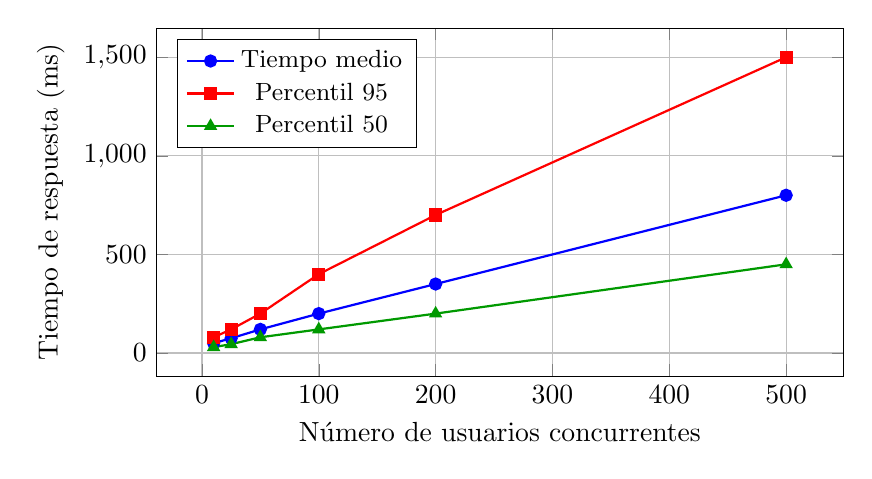
\begin{tikzpicture}
    \begin{axis}[
      xlabel={Número de usuarios concurrentes},
      ylabel={Tiempo de respuesta (ms)},
      grid=major,
      width=0.85\textwidth,
      height=6cm,
      legend pos=north west,
      legend style={font=\small},
    ]
    \addplot[blue, mark=*, thick] coordinates {
      (10, 50) (25, 75) (50, 120) (100, 200) (200, 350) (500, 800)
    };
    \addlegendentry{Tiempo medio}
    
    \addplot[red, mark=square*, thick] coordinates {
      (10, 80) (25, 120) (50, 200) (100, 400) (200, 700) (500, 1500)
    };
    \addlegendentry{Percentil 95}
    
    \addplot[green!60!black, mark=triangle*, thick] coordinates {
      (10, 30) (25, 45) (50, 80) (100, 120) (200, 200) (500, 450)
    };
    \addlegendentry{Percentil 50}
    \end{axis}
  \end{tikzpicture}
  \caption{Tiempos de respuesta según carga de usuarios}
  \label{fig:rendimiento}
\end{figure}

Como se observa en la Figura~\ref{fig:rendimiento}, el sistema mantiene tiempos de respuesta aceptables incluso con 200 usuarios concurrentes.

\subsection{Gráfica de barras}

\begin{figure}[H]
  \centering
  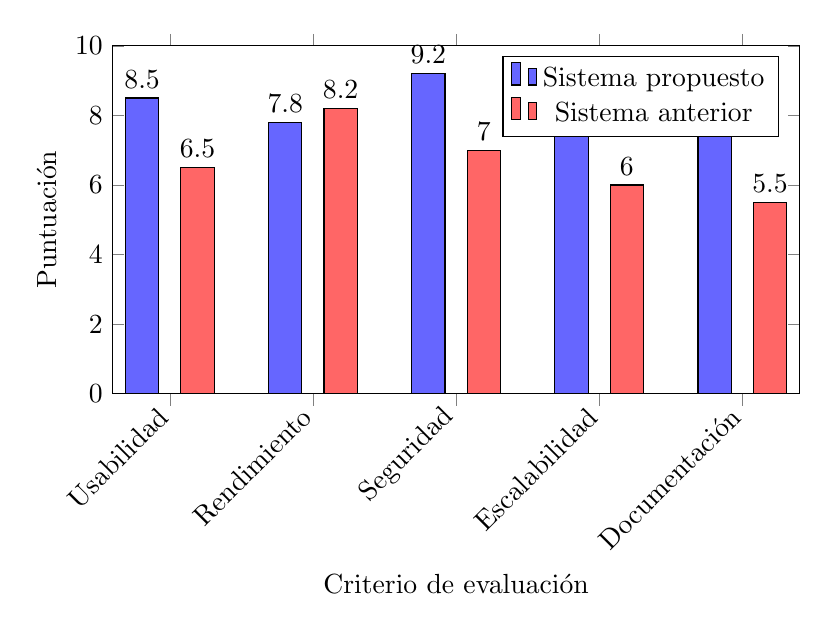
\begin{tikzpicture}
    \begin{axis}[
      ybar=8pt,
      width=0.85\textwidth,
      height=6cm,
      ylabel={Puntuación},
      xlabel={Criterio de evaluación},
      symbolic x coords={Usabilidad, Rendimiento, Seguridad, Escalabilidad, Documentación},
      xtick=data,
      x tick label style={rotate=45, anchor=east},
      ymin=0,
      ymax=10,
      bar width=12pt,
      legend pos=north east,
      nodes near coords,
      nodes near coords align={vertical},
    ]
    \addplot[fill=blue!60] coordinates {
      (Usabilidad, 8.5)
      (Rendimiento, 7.8)
      (Seguridad, 9.2)
      (Escalabilidad, 7.5)
      (Documentación, 8.0)
    };
    \addlegendentry{Sistema propuesto}
    
    \addplot[fill=red!60] coordinates {
      (Usabilidad, 6.5)
      (Rendimiento, 8.2)
      (Seguridad, 7.0)
      (Escalabilidad, 6.0)
      (Documentación, 5.5)
    };
    \addlegendentry{Sistema anterior}
    \end{axis}
  \end{tikzpicture}
  \caption{Comparativa de evaluación del sistema}
  \label{fig:barras}
\end{figure}

\subsection{Gráfica circular (pie chart)}

\begin{figure}[H]
  \centering
  \begin{tikzpicture}
    \pie[
      text=legend,
      radius=2.5,
      color={blue!60, red!60, green!60, orange!60, purple!60}
    ]{
      35/Desarrollo,
      25/Análisis,
      20/Pruebas,
      12/Documentación,
      8/Reuniones
    }
  \end{tikzpicture}
  \caption{Distribución del tiempo del proyecto}
  \label{fig:pie}
\end{figure}

\subsection{Gráfica de área}

\begin{figure}[H]
  \centering
  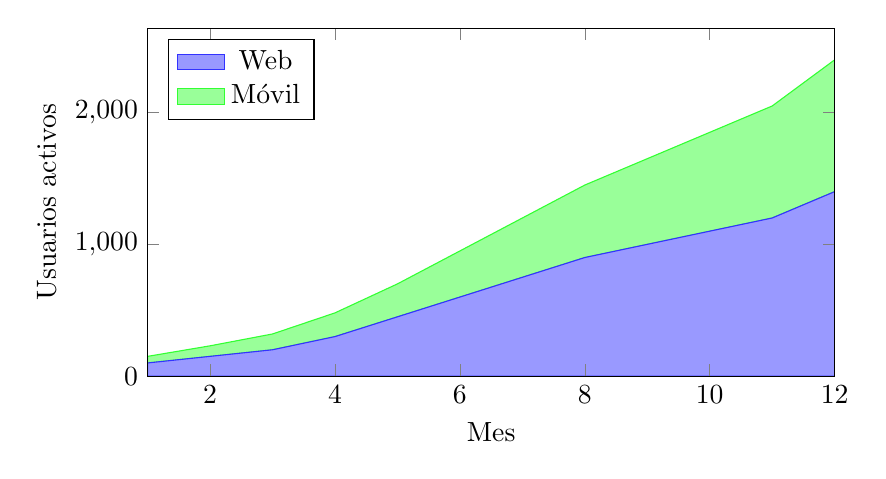
\begin{tikzpicture}
    \begin{axis}[
      width=0.85\textwidth,
      height=6cm,
      xlabel={Mes},
      ylabel={Usuarios activos},
      xmin=1, xmax=12,
      ymin=0,
      area style,
      stack plots=y,
      legend pos=north west,
    ]
    \addplot+[fill=blue!40, draw=blue!80] coordinates {
      (1,100) (2,150) (3,200) (4,300) (5,450) (6,600)
      (7,750) (8,900) (9,1000) (10,1100) (11,1200) (12,1400)
    } \closedcycle;
    \addlegendentry{Web}
    
    \addplot+[fill=green!40, draw=green!80] coordinates {
      (1,50) (2,80) (3,120) (4,180) (5,250) (6,350)
      (7,450) (8,550) (9,650) (10,750) (11,850) (12,1000)
    } \closedcycle;
    \addlegendentry{Móvil}
    \end{axis}
  \end{tikzpicture}
  \caption{Evolución de usuarios activos por plataforma}
  \label{fig:area}
\end{figure}

\subsection{Gráfica de dispersión}

\begin{figure}[H]
  \centering
  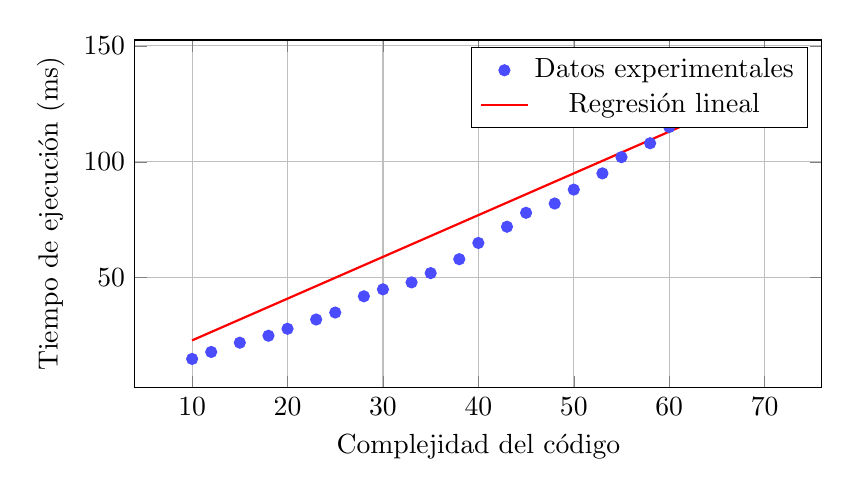
\begin{tikzpicture}
    \begin{axis}[
      width=0.85\textwidth,
      height=6cm,
      xlabel={Complejidad del código},
      ylabel={Tiempo de ejecución (ms)},
      grid=major,
    ]
    \addplot[only marks, mark=*, blue!70, mark size=2pt] coordinates {
      (10,15) (15,22) (20,28) (25,35) (30,45) (35,52)
      (40,65) (45,78) (50,88) (55,102) (60,115) (65,130)
      (12,18) (18,25) (23,32) (28,42) (33,48) (38,58)
      (43,72) (48,82) (53,95) (58,108) (63,122) (68,140)
    };
    
    \addplot[red, thick, domain=10:70] {1.8*x + 5};
    \addlegendentry{Datos experimentales}
    \addlegendentry{Regresión lineal}
    \end{axis}
  \end{tikzpicture}
  \caption{Correlación entre complejidad y tiempo de ejecución}
  \label{fig:scatter}
\end{figure}

\section{Resultados de la implementación}

\subsection{Funcionalidades implementadas}

Se han implementado con éxito las siguientes funcionalidades:

\begin{table}[H]
  \centering
  \caption{Estado de implementación de funcionalidades}
  \label{tab:funcionalidades}
  \begin{tabular}{@{}lcc@{}}
    \toprule
    \textbf{Funcionalidad} & \textbf{Estado} & \textbf{Cobertura tests} \\
    \midrule
    Autenticación de usuarios & Completado & 95\% \\
    Gestión de datos & Completado & 88\% \\
    Generación de informes & Completado & 82\% \\
    API REST & Completado & 90\% \\
    Interfaz de usuario & Completado & 75\% \\
    Sistema de caché & Completado & 85\% \\
    \bottomrule
  \end{tabular}
\end{table}

\subsection{Consumo de recursos}

El consumo de memoria se mantiene estable, como muestra la siguiente ecuación para el consumo estimado:

\begin{equation}
  M_{total} = M_{base} + n \cdot M_{usuario}
  \label{eq:memoria}
\end{equation}

\begin{condiciones}
  M_{total} & = & memoria total consumida (MB) \\
  M_{base}  & = & memoria base del sistema (256 MB) \\
  n         & = & número de usuarios activos \\
  M_{usuario} & = & memoria por usuario (2.5 MB)
\end{condiciones}

\section{Análisis de resultados}

\subsection{Cumplimiento de objetivos}

En la Tabla~\ref{tab:objetivos} se muestra el grado de cumplimiento de cada objetivo:

\begin{table}[H]
  \centering
  \caption{Cumplimiento de objetivos}
  \label{tab:objetivos}
  \begin{tabular}{@{}lp{6cm}c@{}}
    \toprule
    \textbf{Objetivo} & \textbf{Descripción} & \textbf{Cumplimiento} \\
    \midrule
    OE1 & Análisis del estado actual & 100\% \\
    OE2 & Diseño de arquitectura escalable & 100\% \\
    OE3 & Implementación de componentes & 95\% \\
    OE4 & Evaluación del sistema & 100\% \\
    OE5 & Documentación completa & 100\% \\
    \bottomrule
  \end{tabular}
\end{table}

\subsection{Métricas de rendimiento}

\begin{table}[H]
  \centering
  \caption{Métricas de rendimiento del sistema}
  \label{tab:metricas}
  \begin{tabular}{@{}lccc@{}}
    \toprule
    \textbf{Métrica} & \textbf{Objetivo} & \textbf{Resultado} & \textbf{Estado} \\
    \midrule
    Tiempo de respuesta medio & < 200 ms & 145 ms & \textcolor{green!60!black}{\checkmark} \\
    Tiempo de respuesta P95 & < 500 ms & 380 ms & \textcolor{green!60!black}{\checkmark} \\
    Throughput & > 1000 req/s & 1250 req/s & \textcolor{green!60!black}{\checkmark} \\
    Disponibilidad & > 99.5\% & 99.8\% & \textcolor{green!60!black}{\checkmark} \\
    Uso de CPU (promedio) & < 70\% & 45\% & \textcolor{green!60!black}{\checkmark} \\
    Uso de memoria & < 80\% & 62\% & \textcolor{green!60!black}{\checkmark} \\
    \bottomrule
  \end{tabular}
\end{table}

\section{Ejemplo de gráfica 3D}

PGFPlots también permite crear gráficas tridimensionales:

\begin{figure}[H]
  \centering
  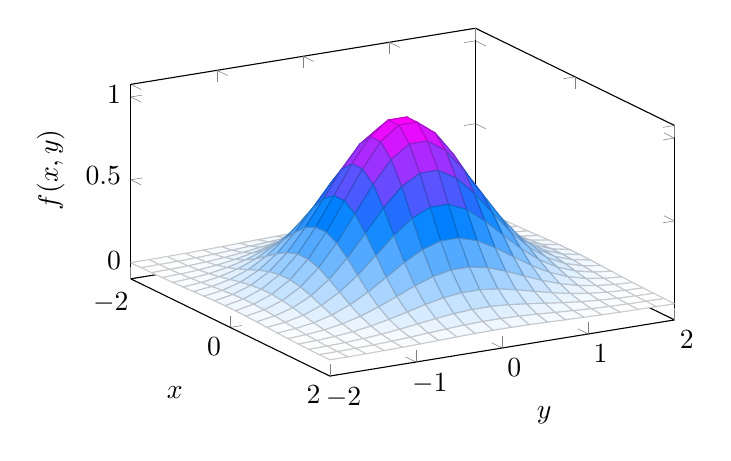
\begin{tikzpicture}
    \begin{axis}[
      width=0.7\textwidth,
      height=6cm,
      view={60}{30},
      xlabel=$x$,
      ylabel=$y$,
      zlabel={$f(x,y)$},
      colormap/cool,
    ]
    \addplot3[
      surf,
      samples=20,
      domain=-2:2,
    ] {exp(-x^2-y^2)};
    \end{axis}
  \end{tikzpicture}
  \caption{Superficie gaussiana $f(x,y) = e^{-x^2-y^2}$}
  \label{fig:3d}
\end{figure}

\section{Exportar gráficas desde herramientas externas}

También es posible exportar gráficas desde otras herramientas:

\begin{itemize}
  \item \textbf{MATLAB:} Usar \texttt{matlab2tikz} para exportar figuras
  \item \textbf{Python (matplotlib):} Usar \texttt{tikzplotlib}
  \item \textbf{R:} Usar el paquete \texttt{tikzDevice}
  \item \textbf{GeoGebra:} Exportar directamente a TikZ
\end{itemize}

\begin{latexcode}[title={Ejemplo de uso de matlab2tikz}]
% En MATLAB:
plot(x, y);
matlab2tikz('figura.tex');

% En LaTeX:
\begin{figure}[H]
  \centering
  \input{figuras/figura.tex}
  \caption{Gráfica importada de MATLAB}
\end{figure}
\end{latexcode}

\section{Gráficas con marcadores y anotaciones}

\subsection{Gráfica con marcadores sobre puntos específicos}

\begin{figure}[H]
  \centering
  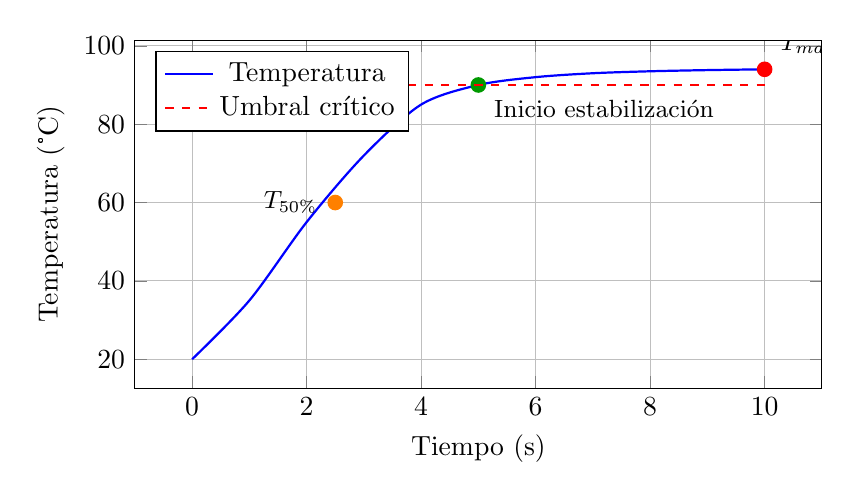
\begin{tikzpicture}
    \begin{axis}[
      width=0.85\textwidth,
      height=6cm,
      xlabel={Tiempo (s)},
      ylabel={Temperatura (°C)},
      grid=major,
      legend pos=north west,
    ]
    % Curva principal
    \addplot[blue, thick, smooth] coordinates {
      (0,20) (1,35) (2,55) (3,72) (4,85) (5,90) (6,92) (7,93) (8,93.5) (9,93.8) (10,94)
    };
    \addlegendentry{Temperatura}
    
    % Marcadores con anotaciones
    \node[circle, fill=red, inner sep=2pt, label={above right:\small $T_{max}=94°C$}] at (axis cs:10,94) {};
    \node[circle, fill=green!60!black, inner sep=2pt, label={below right:\small Inicio estabilización}] at (axis cs:5,90) {};
    \node[circle, fill=orange, inner sep=2pt, label={left:\small $T_{50\%}$}] at (axis cs:2.5,60) {};
    
    % Línea de referencia
    \addplot[dashed, red, thick] coordinates {(0,90) (10,90)};
    \addlegendentry{Umbral crítico}
    \end{axis}
  \end{tikzpicture}
  \caption{Curva de calentamiento con puntos críticos marcados}
  \label{fig:marcadores}
\end{figure}

\subsection{Gráfica con barras de error}

\begin{figure}[H]
  \centering
  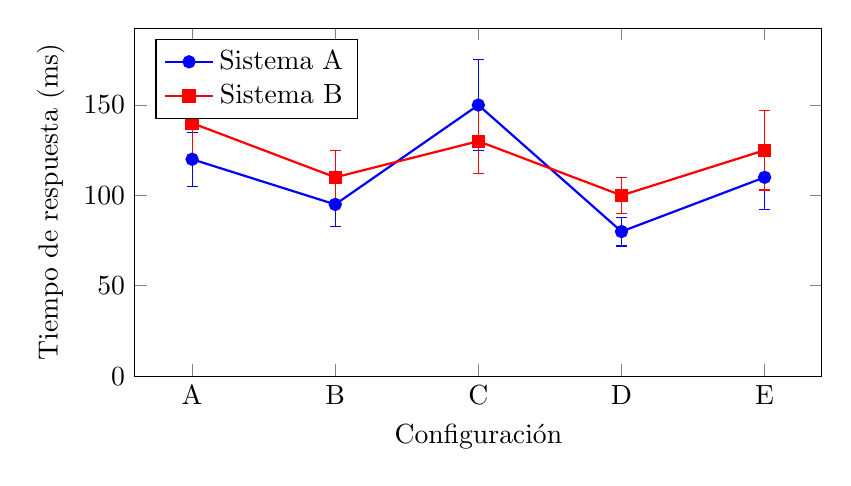
\begin{tikzpicture}
    \begin{axis}[
      width=0.85\textwidth,
      height=6cm,
      xlabel={Configuración},
      ylabel={Tiempo de respuesta (ms)},
      symbolic x coords={A, B, C, D, E},
      xtick=data,
      ymin=0,
      legend pos=north west,
    ]
    % Datos con barras de error
    \addplot[
      blue,
      mark=*,
      thick,
      error bars/.cd,
      y dir=both,
      y explicit,
    ] coordinates {
      (A, 120) +- (0, 15)
      (B, 95) +- (0, 12)
      (C, 150) +- (0, 25)
      (D, 80) +- (0, 8)
      (E, 110) +- (0, 18)
    };
    \addlegendentry{Sistema A}
    
    \addplot[
      red,
      mark=square*,
      thick,
      error bars/.cd,
      y dir=both,
      y explicit,
    ] coordinates {
      (A, 140) +- (0, 20)
      (B, 110) +- (0, 15)
      (C, 130) +- (0, 18)
      (D, 100) +- (0, 10)
      (E, 125) +- (0, 22)
    };
    \addlegendentry{Sistema B}
    \end{axis}
  \end{tikzpicture}
  \caption{Comparativa de rendimiento con intervalos de confianza}
  \label{fig:errorbars}
\end{figure}

\subsection{Gráfica con área sombreada (intervalo de confianza)}

\begin{figure}[H]
  \centering
  \begin{tikzpicture}
    \begin{axis}[
      width=0.85\textwidth,
      height=6cm,
      xlabel={Iteración},
      ylabel={Precisión (\%)},
      grid=major,
      legend pos=south east,
    ]
    % Área de confianza (sombra)
    \addplot[
      name path=upper,
      draw=none,
    ] coordinates {
      (1,72) (2,78) (3,83) (4,87) (5,90) (6,92) (7,93) (8,94) (9,94.5) (10,95)
    };
    
    \addplot[
      name path=lower,
      draw=none,
    ] coordinates {
      (1,62) (2,68) (3,73) (4,77) (5,80) (6,82) (7,83) (8,84) (9,84.5) (10,85)
    };
    
    \addplot[blue!20] fill between[of=upper and lower];
    
    % Curva media
    \addplot[blue, thick, mark=*, mark size=1.5pt] coordinates {
      (1,67) (2,73) (3,78) (4,82) (5,85) (6,87) (7,88) (8,89) (9,89.5) (10,90)
    };
    \addlegendentry{Media $\pm$ desv. estándar}
    \end{axis}
  \end{tikzpicture}
  \caption{Evolución del entrenamiento con banda de confianza}
  \label{fig:confidence}
\end{figure}

\subsection{Gráfica con múltiples ejes Y}

\begin{figure}[H]
  \centering
  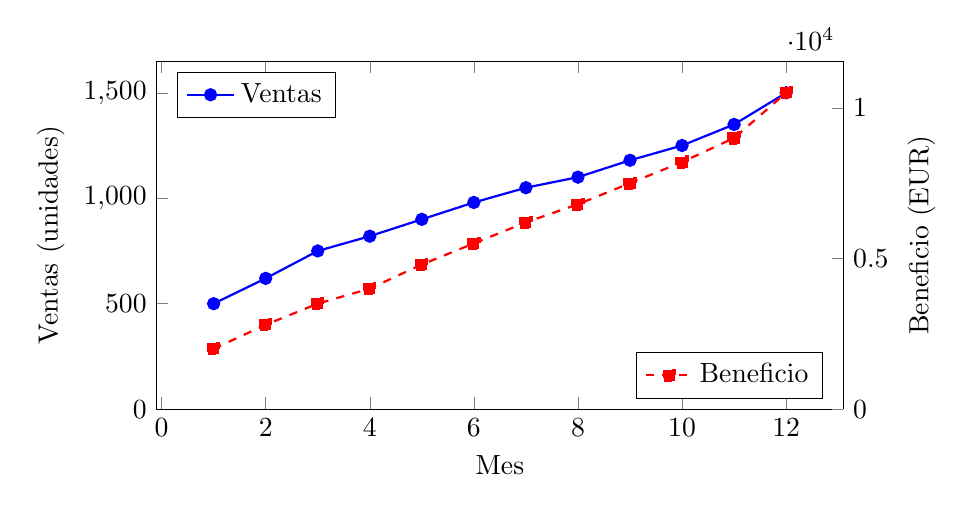
\begin{tikzpicture}
    \begin{axis}[
      width=0.85\textwidth,
      height=6cm,
      xlabel={Mes},
      ylabel={Ventas (unidades)},
      axis y line*=left,
      ymin=0,
      legend pos=north west,
    ]
    \addplot[blue, thick, mark=*] coordinates {
      (1,500) (2,620) (3,750) (4,820) (5,900) (6,980)
      (7,1050) (8,1100) (9,1180) (10,1250) (11,1350) (12,1500)
    };
    \addlegendentry{Ventas}
    \end{axis}
    
    \begin{axis}[
      width=0.85\textwidth,
      height=6cm,
      ylabel={Beneficio (EUR)},
      axis y line*=right,
      axis x line=none,
      ymin=0,
      legend pos=south east,
    ]
    \addplot[red, thick, mark=square*, dashed] coordinates {
      (1,2000) (2,2800) (3,3500) (4,4000) (5,4800) (6,5500)
      (7,6200) (8,6800) (9,7500) (10,8200) (11,9000) (12,10500)
    };
    \addlegendentry{Beneficio}
    \end{axis}
  \end{tikzpicture}
  \caption{Ventas y beneficios mensuales (doble eje Y)}
  \label{fig:dualaxis}
\end{figure}

\subsection{Gráfica de distribución (histograma)}

\begin{figure}[H]
  \centering
  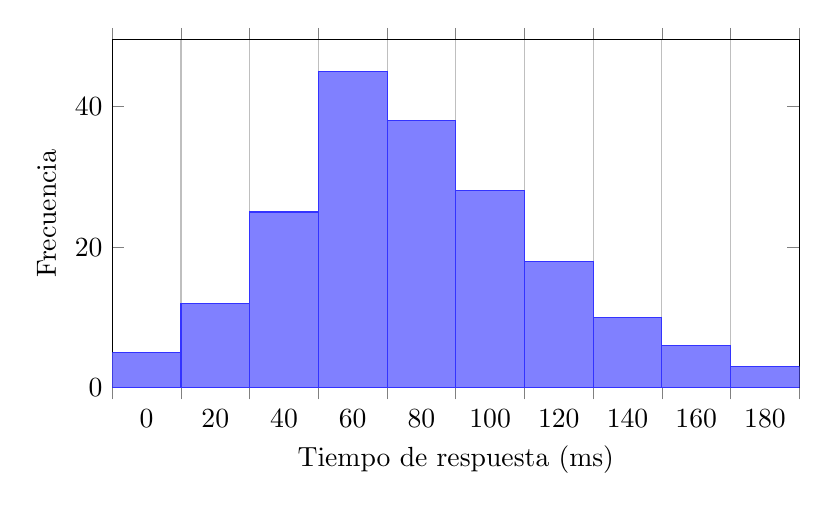
\begin{tikzpicture}
    \begin{axis}[
      width=0.85\textwidth,
      height=6cm,
      ybar interval,
      xlabel={Tiempo de respuesta (ms)},
      ylabel={Frecuencia},
      xmin=0, xmax=200,
      ymin=0,
    ]
    \addplot[fill=blue!50, draw=blue!80] coordinates {
      (0,5) (20,12) (40,25) (60,45) (80,38) 
      (100,28) (120,18) (140,10) (160,6) (180,3) (200,0)
    };
    \end{axis}
  \end{tikzpicture}
  \caption{Distribución de tiempos de respuesta}
  \label{fig:histograma}
\end{figure}

\subsection{Gráfica de radar (polígono)}

Las gráficas de radar son útiles para comparar múltiples variables simultáneamente:

\begin{figure}[H]
  \centering
  \begin{tikzpicture}
    \begin{polaraxis}[
      width=8cm,
      xtick={0,60,120,180,240,300},
      xticklabels={Usabilidad,Rendimiento,Seguridad,Escalabilidad,Mantenibilidad,Portabilidad},
      ymin=0, ymax=100,
      ytick={20,40,60,80,100},
      ylabel near ticks,
      legend pos=outer north east,
    ]
    % Sistema A
    \addplot[blue, thick, fill=blue!20, opacity=0.7] coordinates {
      (0,85) (60,72) (120,90) (180,68) (240,78) (300,82) (360,85)
    };
    \addlegendentry{Sistema A}
    
    % Sistema B
    \addplot[red, thick, fill=red!20, opacity=0.5] coordinates {
      (0,75) (60,88) (120,70) (180,85) (240,72) (300,68) (360,75)
    };
    \addlegendentry{Sistema B}
    \end{polaraxis}
  \end{tikzpicture}
  \caption{Comparativa de sistemas mediante gráfica de radar}
  \label{fig:radar}
\end{figure}

\subsection{Diagrama de Gantt simplificado}

Para mostrar cronogramas de proyecto:

\begin{figure}[H]
  \centering
  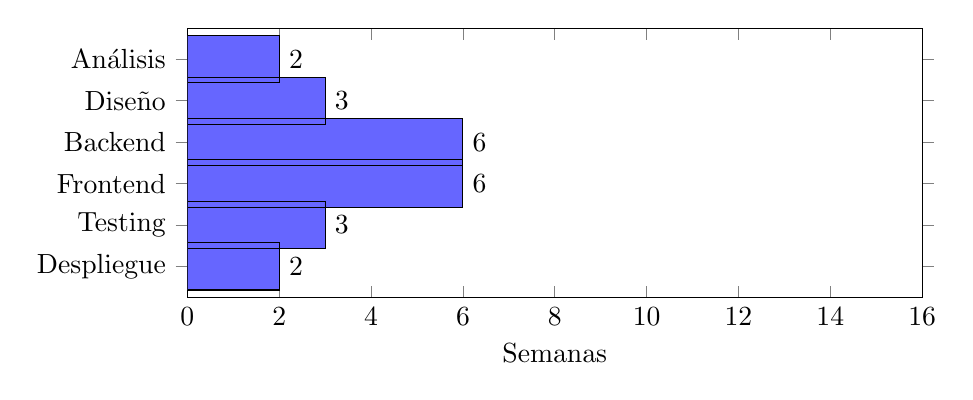
\begin{tikzpicture}
    \begin{axis}[
      width=0.9\textwidth,
      height=5cm,
      xbar,
      xlabel={Semanas},
      ytick={1,2,3,4,5,6},
      yticklabels={Despliegue,Testing,Frontend,Backend,Diseño,Análisis},
      xmin=0, xmax=16,
      bar width=0.6cm,
      nodes near coords,
      nodes near coords align={horizontal},
      enlarge y limits=0.15,
    ]
    % Duración de cada tarea (inicio implícito desde 0 para simplificar)
    \addplot[fill=blue!60] coordinates {(2,6) (3,5) (6,4) (6,3) (3,2) (2,1)};
    \end{axis}
  \end{tikzpicture}
  \caption{Diagrama de Gantt simplificado del proyecto}
  \label{fig:gantt-simple}
\end{figure}

\section{Tabla de resumen de resultados}

Para finalizar, es común presentar un resumen numérico de los resultados:

\begin{table}[H]
  \centering
  \caption{Resumen de métricas de evaluación}
  \label{tab:resumen-metricas}
  \begin{tabular}{@{}lccccc@{}}
    \toprule
    \textbf{Métrica} & \textbf{Baseline} & \textbf{Propuesta} & \textbf{Mejora} & \textbf{p-valor} & \textbf{Sig.} \\
    \midrule
    Precisión & 78.5\% & 89.2\% & +10.7\% & 0.001 & *** \\
    Recall & 72.3\% & 86.8\% & +14.5\% & 0.003 & ** \\
    F1-Score & 75.2\% & 87.9\% & +12.7\% & 0.002 & ** \\
    Tiempo (ms) & 145 & 98 & -32.4\% & 0.015 & * \\
    Memoria (MB) & 512 & 384 & -25.0\% & 0.042 & * \\
    \bottomrule
  \end{tabular}
  
  \medskip
  \footnotesize
  Significancia: *** p < 0.001, ** p < 0.01, * p < 0.05
\end{table}
